%; whizzy chapter
% -initex iniptex -latex platex -format platex -bibtex jbibtex -fmt fmt
% $B0J>e(B whizzytex $B$r;HMQ$9$k>l9g$N@_Dj!#(B


%     Tokyo Debian Meeting resources
%     Copyright (C) 2006 Junichi Uekawa

%     This program is free software; you can redistribute it and/or modify
%     it under the terms of the GNU General Public License as published by
%     the Free Software Foundation; either version 2 of the License, or
%     (at your option) any later version.

%     This program is distributed in the hope that it will be useful,
%     but WITHOUT ANY WARRANTY; without even the implied warranty of
%     MERCHANTABILITY or FITNESS FOR A PARTICULAR PURPOSE.  See the
%     GNU General Public License for more details.

%     You should have received a copy of the GNU General Public License
%     along with this program; if not, write to the Free Software
%     Foundation, Inc., 51 Franklin St, Fifth Floor, Boston, MA  02110-1301 USA


%   Pdf$B:n@.<j=g(B
% dvipdfmx debianmeetingresume200607.dvi
%  preview (shell-command (concat "xpdf " (replace-regexp-in-string "tex$" "pdf"(buffer-file-name)) "&"))
% $B2hA|%U%!%$%k$r=hM}$9$k$?$a$K$O(Bebb$B$rMxMQ$7$F(Bboundingbox$B$r:n@.!#(B
%(shell-command "cd image200607; ebb *.png")

%%$B$3$3$+$i%X%C%@3+;O!#(B

\documentclass[mingoth,a4paper]{jsarticle}
\usepackage[dvipdfm]{graphicx}
\usepackage{fancybox}
\usepackage{longtable}
\usepackage{ascmac}	% $B0O$_(B (screen,itembox)
\usepackage{fancyvrb}   % $B0O$_(B Verbatim $B$N$?$a$KI,MW(B
\usepackage[dvipdfm]{hyperref}
\usepackage{url}
\usepackage[dvipdfm]{color}

%http://www.naney.org/diki/dk/hyperref.html
%$BF|K\8l(BEUC$B7O4D6-$N;~(B
\AtBeginDvi{\special{pdf:tounicode EUC-UCS2}}
%$B%7%U%H(BJIS$B7O4D6-$N;~(B
%\AtBeginDvi{\special{pdf:tounicode 90ms-RKSJ-UCS2}}

%% spacing $B$N@_Dj$r$9$k!#30OH$r8:$i$9!#(B
\setlength\headheight{0mm}
\setlength\topmargin{-20mm}
\setlength\headsep{0mm}
\setlength\topskip{3mm}
\setlength\maxdepth{4pt}
\setlength\columnsep{6mm}
\setlength\textheight{252mm}
\setlength\topmargin{-5mm}
\setlength\textwidth{170mm}
\setlength\oddsidemargin{-5mm}
\setlength\evensidemargin{-5mm}

% commandline$B4D6-$rDj5A!#2hLLF~=PNO$K$D$$$F$O(Bcommandline$B4D6-(B
% $B$GI=5-$9$k(B
\newenvironment{commandline}%
{\VerbatimEnvironment
  \begin{Sbox}\begin{minipage}{15cm}\begin{fontsize}{7.3}{7.3} \begin{BVerbatim}}%
{\end{BVerbatim}\end{fontsize}\end{minipage}\end{Sbox}
  \setlength{\fboxsep}{8pt}\fbox{\TheSbox}}


%%% start of santaku
\makeatletter
\newwrite\tf@jqz
\immediate\openout\tf@jqz\jobname.jqz\relax
\makeatother
\newcounter{santakucounter}
\newcommand{\santaku}[5]{%
\addtocounter{santakucounter}{1}

\addtocontents{jqz}{\arabic{santakucounter}. #5\\}
\begin{minipage}{1\hsize}
$BLdBj(B\arabic{santakucounter}. 
#1\\
$B""(B A #2\\
$B""(B B #3\\
$B""(B C #4
\end{minipage}
\hspace{1cm}
\\

}
%%% end of santaku

\newcommand{\emptyspace}{(\underline{\hspace{1cm}})}

\newcommand{\subsubsubsection}[1]{%
\vspace{1zw}{\bf #1}\\}


% section$B$r%;%s%?%j%s%0$9$k(B
\makeatletter
  \renewcommand{\section}{\@startsection{section}{1}{\z@}%
    {\Cvs \@plus.5\Cdp \@minus.2\Cdp}% $BA0%"%-(B
    {.5\Cvs \@plus.3\Cdp}% $B8e%"%-(B
    {\normalfont\Huge\headfont\raggedright\centering}} % style
\makeatother

% section $B$NBe$o$j$N4D6-(B
\newcommand{\dancersection}[2]{%
\newpage
$BEl5~%(%j%"(BDebian$BJY6/2q(B 2006
\hrule
\vspace{0.5mm}
\hrule
%\hfill{}
\includegraphics[width=3cm]{image200502/openlogo-nd.eps}\\
\hfill{}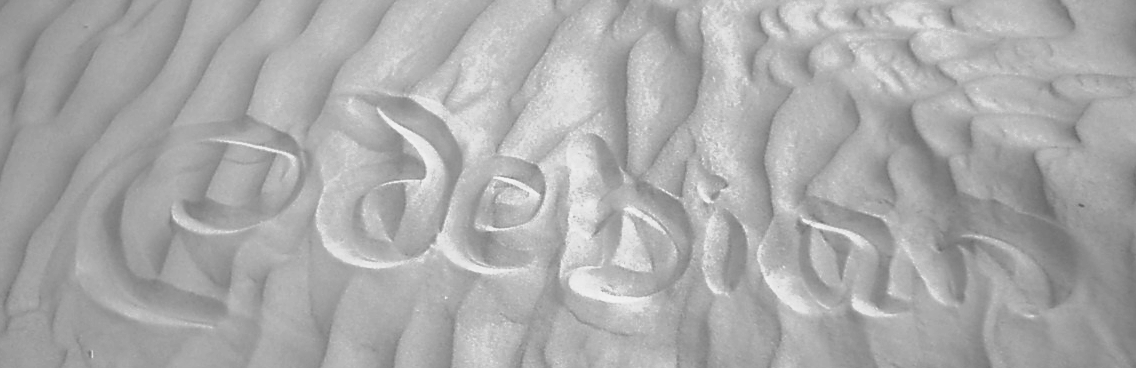
\includegraphics[width=16cm]{image2006-natsu/guruguru-sand-light.png}\\
\vspace{-5cm}
\begin{center}
\section{#1}
\end{center}
\hfill{}\colorbox{white}{#2}\hspace{3cm}\space\\
\vspace{1cm}
\hrule
\vspace{0.5mm}
\hrule
\vspace{1cm}
}

% BTS$B$NHV9f$r8+$k$?$a$N%3%^%s%I(B
\newcommand{\debianbug}[1]{#1\footnote{\url{http://bugs.debian.org/#1}}}

% for dancerj
\newcommand{\fgref}[1]{$B?^(B\ref{#1}}
\newcommand{\tbref}[1]{$BI=(B\ref{#1}}


\begin{document}

\begin{titlepage}

% $BKh7nJQ99$9$kItJ,(B, $BK\J8$NKvHx$b=$@5$9$k$3$H$r$o$9$l$:$K(B
\title{
\includegraphics[width=7cm]{image200502/openlogo-nd.eps}\\
 $BBh(B18$B2s(B $BEl5~%(%j%"(B Debian $BJY6/2q(B\\$B;vA0;qNA(B}
\date{2006$BG/(B7$B7n(B15$BF|(B}
\author{Debian$BJY6/2q2q>l78(B $B>e@n=c0l(B\thanks{Debian Project Official Developer}} 
\maketitle
\thispagestyle{empty}
\end{titlepage}

\newpage
\tableofcontents

\dancersection{Introduction To Debian $BJY6/2q(B}{$B>e@n=c0l(B}

$B:#7n$N(BDebian$BJY6/2q$X$h$&$3$=!#(B
$B$3$l$+$i(BDebian$B$N$"$d$7$$@$3&$KF~$k$H$$$&J}$b!"$9$G$K$I$C$W$j$H$D$+$C$F$$(B
$B$k$H$$$&J}$b!"7n$K0l2s(BDebian$B$K$D$$$F8l$j$^$;$s$+!)(B

$BL\E*$H$7$F2<5-$NFs$D$r9M$($F$$$^$9!#(B

\begin{itemize}
 \item $B%a!<%k$G$O$h$_$H$l$J$$!"$b$7$/$O$h$_$H$C$F$i$l$J$$$h$&$J>pJs$r>p(B
       $BJs6&M-$9$k>l$r$D$/$k(B
 \item $B$^$H$^$C$F$$$J$$(BDebian$B$rMxMQ$9$k:]$N>pJs$r$^$H$a$F!"$"$kDxEY$N2t$H(B
       $B$7$F=P$7$F$_$k(B
\end{itemize}

$B$^$?!"El5~$K$O(BLinux$B$NJY6/2q$O$?$/$5$s$"$j$^$9$N$G!"(BDebian$B$K8BDj$7$?JY6/(B
$B2q$K$7$^$9!#(BLinux$B$N4pK\E*$JMxMQJ}K!$J$I$,CN$j$?$$J}$O!"B>$G$,$s$P$C$F$/$@$5(B
$B$$!#(B
Debian$B$NJY6/2q$H$$$&$3$H$G5f6KE*$K$O;22C<TA40w$,(BDebian Package$B$r(B
$B$,$j$,$j$H:n$j$J$,$i%9!<%Q!<%O%C%+!<$K$J$l$k$h$&$J;Q$rLQA[$7$F$$$^$9!#(B

Debian$B$r$3$l$+$i$I$&$9$k$H$$$&G=F0E*$JE83+$X$NEZBf$H$7$F$N6u4V$rDs6!$7!"(B
$B>pJs$N6&M-$r$7$?$$!"$H$$$&$N$,L\E*$G$9!#(B
$B<!2s$O0c$&$3$H8@$C$F$k$+$b$7$l$^$;$s$,!"8fMF<O$r!#(B

\subsection{$B9V;U>R2p(B}

\begin{itemize}
 \item{$B4d>>$5$s(B} $BK]Lu$N%$%s%U%i$K$D$$$F>R2p$7$^$9!#(B
 \item{$B>e@n=c0l(B} $B1c2q$N44;v$G$9!#(B
\end{itemize}

\subsection{$B;vA02]Bj>R2p(B}

$B:#2s$N;vA02]Bj$O(B
$B!V:#2s<B8=$9$k$3$H!W(B
$B$H$$$&%?%$%H%k$G(B200-800$BJ8;zDxEY$NJ8>O$r=q$$$F$/$@$5$$!#(B
$B$H$$$&$b$N$G$7$?!#(B
$B$=$N2]Bj$KBP$7$F2<5-$NFbMF$rDs=P$$$?$@$-$^$7$?!#(B

\subsubsection{$B4d>>$5$s(B}

$B%8%s%.%9%+%s?)$$$^$9!#(B

\subsubsection{$B>e@n(B}

$BKL3$F;$N6u5$$r5[$$$^$9!#(B

\dancersection{$B:G6a$N(BDebian$B4XO"$N%_!<%F%#%s%0Js9p(B}{$B>e@n=c0l(B}

\subsection{$BEl5~%(%j%"(BDebian$BJY6/2q(B17$B2sL\Js9p(B}
% (query-replace-regexp "<.*>" "")

$BEl5~%(%j%"(BDebian$BJY6/2qJs9p!%(B6$B7n$NBh(B17$B2s(BDebian$BJY6/2q$r<B;\$7$^$7$?!%4d>>(B
$B$5$s$,(BDebian Conference $B$NJs9p$r$7$^$7$?!%>e@n$,(B cowbuilder $B$N;H$$J}$K$D(B
$B$$$FH/I=$7$^$7$?!%(B
	  
$B:#2s$N;22C?M?t$O(B16$B?M$G$7$?!%(B
	  
$B:G=i$O;vA02]Bj$NH/I=!%$_$J$5$s(B Debconf $B$K;22C$9$k$J$i!$N"J}$r<jEA$$$^$9!$(B
$B$H$$$&0U8+$,B?$+$C$?$h$&$G$9!%4d>>$5$s$O(BFlash$B$N(BBOF$B$r3+:E$9$k$H$N$3$H$G!$(B
$BMhG/$K4|BT$G$9!%(B

Debian weekly news quiz $B$O$"$1$I$5$s$,K~E@$r$H$j$^$7$?!%$*$a$G$H$&$4$6$$(B
$B$^$9!%>.NS$5$s$O0lLdIT@52r$@$C$?$h$&$G$9!%;DG0!%(B
	  	  
$B4d>>$5$s$,(B Debconf $B$K$D$$$FH/I=!%%;%C%7%g%s$N>R2p$J$I$r$7$^$7$?!%(B
	  
$B>e@n$,(B\texttt{pbuilder/cowdancer/cowbuilder}$B$K$D$$$FH/I=$7$^$7$?!%$$$+$K(B
$B9bB.$K$7$?$N$+!$$H$$$&$3$H$rH/I=$7$^$7$?!%$$$^$^$G!$$3$s$J$K4JC1$J$3$H$r(B
$B$9$k$N$K(B2$BJ,$bBT$C$F$$$?$N$G$9$M!$$H$$$&$3$H$K6CX3!$$h$/$_$s$J2fK}$7$F$/(B
$B$l$?!*$H@9$j>e$,$j$^$7$?!%(B
	  
$B1c2q$O!V$$$M$d!W$K$F3+:E!%?);v$NNL$,$9$/$J$/$F!$:G=i$KCmJ8$7$?>&IJ$,=P=*(B
$B$k$h$j$b$O$d$/%i%9%H%*!<%@!<$N;~4V$,Mh$?$j$H$$$m$$$m$HIT<j:]$,$"$j$^$7$?!$(B
$B<:Ni$7$^$7$?!%(B
	  
\dancersection{MacBook $B$K(B Debian $B$r%$%s%9%H!<%k(B}{$B>e@n(B}
\label{dancerjmacbook}

Apple $B$,(B2006$BG/=U$KH/Gd3+;O$7$?(B Intel $B%Y!<%9$N(BMacBook $B$K(B MacOS X $B$H(B Debian $B$r(B
dual-boot $B$G%$%s%9%H!<%k$NN.$l$r>R2p$7$^$9!#(B

MacOS X $B$r:o=|$7$F(BDebian $B$N$_$r%$%s%9%H!<%k$9$kJ}K!$K$D$$$F$O!"$*$=$i$/(B
lilo$B$r(BMBR$B$+$i5/F0$9$k$h$&$K@_Dj$9$l$P:G?7%U%!!<%`%&%'%"$O5/F0$7$F$/$l$^(B
$B$9$,!"8!>Z$7$F$$$^$;$s!#(B

\subsection{$B%$%s%9%H!<%kMQ$K%Q!<%F%#%7%g%s=`Hw(B}

$B9XF~D>8e$N>uBV$G$O!"(BMac OS X $B$,A4It$NNN0h$r@j$a$F$$$^$9!#$=$N!!(BMacOS X 
$B%Q!<%F%#%7%g%s$r=L>.$7!"(BDebian$B$,%$%s%9%H!<%k$G$-$k$h$&$K$7$^$9!#(BMac OS X
$B$O(B20GB$BDxEY$NNN0h$rI,MW$H$9$k$h$&$G$9$N$G!"(B20GB$B$^$G=L>.$7$F$7$^$$$^$7$g$&!#(B

diskutil resizevolume $B%3%^%s%I$G%\%j%e!<%`%5%$%:$rF0E*$KJQ99$9$k$3$H$,$G(B
$B$-$^$9!#(B\footnote{resizevolume$B%3%^%s%I$O(BMac OS X 10.4.6$B$N5!G=3HD%$N$h$&$G$9!#(B}

\begin{commandline}
Mac OS X $ df -h
Filesystem                Size   Used  Avail Capacity  Mounted on
/dev/disk0s2               74G    17G    57G    23%    /
devfs                      95K    95K     0B   100%    /dev
fdesc                     1.0K   1.0K     0B   100%    /dev
<volfs>                   512K   512K     0B   100%    /.vol
automount -nsl [171]        0B     0B     0B   100%    /Network
automount -fstab [179]      0B     0B     0B   100%    /automount/Servers
automount -static [179]     0B     0B     0B   100%    /automount/static
/dev/disk0s1              197M   512B   197M     0%    /efi

Mac OS X $ sudo diskutil resizevolume disk0s2 20G
Started resizing on disk disk0s2 Macintosh HD
Verifying

Resizing Volume
Adjusting Partitions

Finished resizing on disk disk0s2 Macintosh HD
WARNING: You must now reboot!

# diskutil list
/dev/disk0
   #:                   type name               size      identifier
   0:  GUID_partition_scheme                    *74.5 GB  disk0
   1:                    EFI                    200.0 MB  disk0s1
   2:              Apple_HFS Macintosh HD       20.0 GB   disk0s2

\end{commandline}

\subsection{rEFIt$B$N%$%s%9%H!<%k(B}

rEFIt$B$O(BEFI$B@lMQ%V!<%H%m!<%@$G$9!#(B
rEFIt\footnote{\url{http://refit.sourceforge.net/} $B<9I.;~E@$N%P!<%8%g%s(B
$B$O(B0.7$B$G$7$?!#(B} $B%$%a!<%8$r(B MacOS X $B$K%$%s%9%H!<%k$7$^$9!#%$%s%9%H!<%k$9$k(B
$B>l=j$O$I$3$G$b$h$$$N$G$9$,!"%I%-%e%a%s%H$K=>$C$F$_$^$7$g$&!#(B
\texttt{/efi} $B$"$?$j$K%U%!%$%k$rE83+$7!"(B rEFIt $B$K4^$^$l$F$$$k!"(B
\texttt{./enable.sh} $B$r<B9T$7$^$9!#%9%/%j%W%HFbIt$G(B \texttt{bless} $B%3%^(B
$B%s%I(B\footnote{EFI$B$G$N(BOS$B5/F0M%@h=g=x$rJQ99$7$F$/$l$k%D!<%k(B}$B$r<B9T$7$F$/$l(B
$B$^$9!#$3$l$G!"5/F0;~$K<+F0$G(B rEFIt$B!!$,<B9T$5$l$k$h$&$K$J$j$^$9!#(B

Debian$B$N(BrEFIt$B%Q%C%1!<%8$rMxMQ$7$F%$%s%9%H!<%k$9$k>l9g$K$O%P!<%8%g%s(B0.7-3 
$B;~E@$G$O(B enable.sh $B$rDs6!$7$F$$$^$;$s!"D>@\(Bbless$B%3%^%s%I$rF~NO$7$F$/$@$5(B
$B$$!#(B

\texttt{sudo bless --folder \textit{[refit.efi$B$N$"$k%G%#%l%/%H%j$X$N%U%k%Q%9(B]} --file \textit{[refit.efi$B$X$N%U%k%Q%9(B]}}

\begin{center}
  \includegraphics[width=0.5\hsize]{image200607/bootchain.ps}
\end{center}

\subsection{Debian $B$N%$%s%9%H!<%k(B}

2006$BG/(B7$B7nHG0J9_$N(Betch\footnote{$B$3$l0JA0$K$D$$$F$OF0:n3NG'$r$7$F$$$^$;$s!#(B} 
$B$N%$%s%9%H!<%i$rMxMQ$7$F%$%s%9%H!<%k$7$^$9!#(B

CDROM$B$+$i5/F0$9$k$?$a$K$O!"(BCDROM$B$rA^F~$7$F$+$i!"(BC$B$r2!$7$J$,$i5/F0$9$l$P(B
$B$h$$$G$9!#$b$7$/$O!"(Boption $B%-!<$r2!$7$J$,$i5/F0$9$k$H%U%!!<%`%&%'%"$NA*(B
$BBr2hLL$,5/F0$7$^$9!#(BrEFIt$B$N%a%K%e!<$+$i$b(BCDROM$B$+$i$N5/F0$rA*Br$G$-$^$9!#(B
\footnote{2006$BG/(B7$B7n;~E@$G(BDebian Installer$B!!$GMxMQ$7$F$$$k(BLinux $B%+!<%M%k(B 
2.6.15, 2.6.16$B!!$"$?$j$G$O(B Intel Mac $B$KBP1~$G$-$F$$$J$$LdBj$,$"$j!"(B5$B2s$K(B
4$B2sDxEY$O!V(BAPIC$B%(%i!<!W$J$k$b$N$,H/@8$7!"5/F0$K<:GT$9$k$N$G!":,5$$h$/5/(B
$BF0$9$k$^$G$,$s$P$C$F$/$@$5$$!#(B2.6.17 $B0J9_$G$O(BIntel Mac $B8~$1$N=$@5$,0lIt(B
$B%^!<%8$5$l$F$$$k$N$G!">u67$O2~A1$7$F$$$^$9!#(B}

$B%Q!<%F%#%7%g%s$r@Z$kItJ,(B\footnote{$BCm0U;v9`$H$7$F$O!"4{B8$N(BEFI FAT$B$H(BMac
OS X$B$N%Q!<%F%#%7%g%s$O:o=|$7$J$$$3$H!#(BLILO$B$r%$%s%9%H!<%k$9$kM=Dj$N%Q!<%F%#(B
$B%7%g%s$O%Q!<%F%#%7%g%sHV9f!!(B3 $B$+(B 4 $B$K$9$k$3$H!"$H$$$&$3$H$,$"$j$^$9!#(B5$BHV(B
$BL\0J9_$N%Q!<%F%#%7%g%s$O!!(BMBR$B$N@)8B$,$"$k$N$GMxMQ$G$-$^$;$s!#(B}$B$r2a$.!$%Q%C(B
$B%1!<%8$,%$%s%9%H!<%k$5$l$?$i!$(BLILO$B$r%$%s%9%H!<%k$9$kD>A0$NItJ,$^$G<B;\$7(B
$B$^$9!#(B

$B$3$N;~E@$G$O(B LILO $B$,8=:_F0:n$G$-$J$$>uBV$K$J$C$F$$$^$9!#(B\footnote{parted 
$B$,(B GPT $B$N;EMM$K=`5r$7$F$*$j!"(Bpartition 1 $B$N$_$7$+$J$$(B MBR$B>e$N%Q!<%F%#%7%g(B
$B%s%F!<%V%k$r:F:n@.$7$F$$$k$3$H$K$h$k$h$&$G$9!#(B}$B$3$3$G!"(BMBR$B$r(BGPT$B$KF14|$5(B
$B$;$k:n6H$r<B;\$7$^$9!#$3$3$G!"(BAlt-F2 $B$G2>A[%3%s%=!<%k$r@ZBX$(!"%3%^%s%I(B
$B%i%$%s$K$&$D$j$^$9!#(Bgptsync $B%3%^%s%I$r<B9T$7$F$/$@$5$$(B\footnote{$B:#8e$O%$(B
$B%s%9%H!<%i$+$i<B;\$G$-$k$h$&$K2~A1$7$?$$$G$9(B}$B!#(B $B8=>u$N%$%s%9%H!<%kJ}K!$H(B
$B$7$F$O!$(B\texttt{chroot /target bin/sh}$B$H$7$F%$%s%9%H!<%k@h$N(B chroot$B$KF~(B
$B$j!"$=$3$+$i(B \texttt{apt-get install refit} $B$G%Q%C%1!<%8$r%$%s%9%H!<%k!"(B
$B$=$7$F(B\texttt{ gptsync} $B%3%^%s%I$G(BGPT$B$+$i(BMBR$B$KF14|$5$;$^$9!#(B

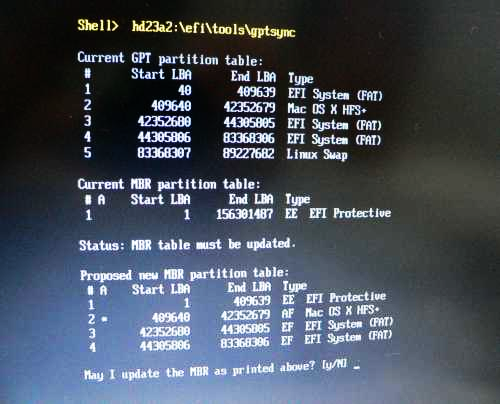
\includegraphics[width=0.9\hsize]{image200607/gptsync.png}

$B$3$N>uBV$G!"%$%s%9%H!<%i$N2hLL$K(B Alt-F1$B$GLa$j!"(BLILO $B$r(B MBR $B$G$O$J$/!"(B
Linux $BMQ$N%Q!<%F%#%7%g%s$K%$%s%9%H!<%k$7$^$9!#:F5/F0$9$k$H(BrEFIt$B$+$i(BLinux
$B$r;XDj$7$F5/F0$G$-$k$h$&$K$J$C$F$$$^$9!#(B

\subsection{$B3F<o%G%P%$%9$N@_Dj(B}
\subsubsection{X$B$N@_Dj(B}

\texttt{X} $B$O(B \texttt{i810} $B%I%i%$%P$G@_Dj$7$^$9!#(B
\texttt{915resolution} $B%Q%C%1!<%8$r%$%s%9%H!<%k$7$^$9!#(B
$B2rA|EY$O(B 1280x800 $B$G$9!#(B

\texttt{/etc/default/915resolution}$B$NNc$G$9!'(B\\
\begin{commandline}
#
# 915resolution default
#
# find free modes by  /usr/sbin/915resolution -l
# and set it to MODE
# e.g. use MODE=54 
MODE=32
#
# and set resolutions for the mode.
# e.g. use XRESO=1024 and YRESO=768
XRESO=1280
YRESO=800
#
# We can also set the pixel mode.
# e.g. use BIT=32
# Please note that this is optional,
# you can also leave this value blank.
BIT=
\end{commandline}

xorg.conf $B$NNc$G$9(B\footnote{$B%G%U%)%k%H$G30It=PNO$b$9$k$h$&$K@_Dj$7$F$"$j$^$9(B}$B!'(B

\begin{commandline}
Section "Files"
	FontPath	"/usr/share/fonts/X11/misc"
	FontPath	"/usr/X11R6/lib/X11/fonts/misc"
	FontPath	"/usr/share/fonts/X11/cyrillic"
	FontPath	"/usr/X11R6/lib/X11/fonts/cyrillic"
	FontPath	"/usr/share/fonts/X11/100dpi/:unscaled"
	FontPath	"/usr/X11R6/lib/X11/fonts/100dpi/:unscaled"
	FontPath	"/usr/share/fonts/X11/75dpi/:unscaled"
	FontPath	"/usr/X11R6/lib/X11/fonts/75dpi/:unscaled"
	FontPath	"/usr/share/fonts/X11/Type1"
	FontPath	"/usr/X11R6/lib/X11/fonts/Type1"
	FontPath	"/usr/share/fonts/X11/100dpi"
	FontPath	"/usr/X11R6/lib/X11/fonts/100dpi"
	FontPath	"/usr/share/fonts/X11/75dpi"
	FontPath	"/usr/X11R6/lib/X11/fonts/75dpi"
	# path to defoma fonts
	FontPath	"/var/lib/defoma/x-ttcidfont-conf.d/dirs/TrueType"
EndSection

Section "Module"
	Load	"i2c"
	Load	"bitmap"
	Load	"ddc"
	Load	"dri"
	Load	"extmod"
	Load	"freetype"
	Load	"glx"
	Load	"int10"
	Load	"type1"
	Load	"vbe"
EndSection


Section "InputDevice"
	Identifier	"Generic Keyboard"
	Driver		"kbd"
	Option		"CoreKeyboard"
	Option		"XkbRules"	"xorg"
	Option		"XkbModel"	"pc104"
	Option		"XkbLayout"	"us"
	Option		"XkbOptions"	"ctrl:nocaps"
EndSection

Section "InputDevice"
	Identifier	"Configured Mouse"
	Driver		"mouse"
	Option		"CorePointer"
	Option		"Device"		"/dev/input/mice"
	Option		"Protocol"		"ExplorerPS/2"
	Option		"Emulate3Buttons"	"true"
EndSection

Section "InputDevice"
	Identifier	"Synaptics Touchpad"
	Driver		"synaptics"
	Option		"SendCoreEvents"	"true"
	Option		"Device"		"/dev/psaux"
	Option		"Protocol"		"auto-dev"
	Option		"HorizScrollDelta"	"0"
EndSection


Section "Device"
	Identifier	"Generic Video Card"
	Driver		"i810"
	Screen		0
	Option "MonitorLayout" "CRT,LFP"
	BusID		"PCI:0:2:0"
EndSection

Section "Device"
	Identifier	"Device1"
	Driver		"i810"
	Screen		1
	Option "MonitorLayout" "CRT,LFP"
	BusID		"PCI:0:2:0"
EndSection

\end{commandline}
\\$BB3$/(B

\begin{commandline}



Section "Monitor"
	Identifier	"Generic Monitor"
	Option		"DPMS"
	HorizSync	28-64
	VertRefresh	43-60
EndSection


Section "Monitor"
	Identifier	"External Monitor"
	Option		"DPMS"
	HorizSync	28-64
	VertRefresh	43-60
EndSection

Section "Screen"
	Identifier	"Default Screen"
	Device		"Generic Video Card"
	Monitor		"Generic Monitor"
	DefaultDepth	24
	SubSection "Display"
		Depth		1
		Modes		"1280x800" "1024x768" "800x600" "640x480"
	EndSubSection
	SubSection "Display"
		Depth		4
		Modes		"1280x800" "1024x768" "800x600" "640x480"
	EndSubSection
	SubSection "Display"
		Depth		8
		Modes		"1280x800" "1024x768" "800x600" "640x480"
	EndSubSection
	SubSection "Display"
		Depth		15
		Modes		"1280x800" "1024x768" "800x600" "640x480"
	EndSubSection
	SubSection "Display"
		Depth		16
		Modes		"1280x800" "1024x768" "800x600" "640x480"
	EndSubSection
	SubSection "Display"
		Depth		24
		Modes		"1280x800" "1024x768" "800x600" "640x480"
	EndSubSection
EndSection

Section "Screen"
	Identifier "Secondary Screen"
	Device "Device1"
	Monitor "External Monitor"
	DefaultDepth 24
	SubSection "Display"
		   Depth 1
		   Modes "1024x768" "800x600"
	EndSubSection
	SubSection "Display"
		   Depth 4
		   Modes "1024x768" "800x600"
	EndSubSection
	SubSection "Display"
		   Depth 8
		   Modes "1024x768" "800x600"
	EndSubSection
	SubSection "Display"
		   Depth 16
		   Modes "1024x768" "800x600"
	EndSubSection
	SubSection "Display"
		   Depth 24
		   Modes "1024x768" "800x600"
	EndSubSection
EndSection

Section "ServerLayout"
	Identifier "Dual-monitor Layout"
	Screen 0 "Default Screen"
	Screen 1 "Secondary Screen" LeftOf "Default Screen"
	# Option "Clone" "On"
	#Option "Xinerama" "On"
	InputDevice "Generic Keyboard"
	InputDevice "Configured Mouse"
	InputDevice "Synaptics Touchpad"
EndSection

Section "DRI"
	Mode	0666
EndSection
 
\end{commandline}

$B%-!<%P%$%s%I$O(B .xsession \footnote{$B:G6a$O%G%U%)%k%H$G$O!!(B.gnomerc$B!!$H$$(B
$B$&%U%!%$%k$,;H$o$l$k$h$&$G$9!#(B GDM$B$+$i%G%U%)%k%H$N%7%9%F%`%;%C%7%g%s$rL@(B
$B<(E*$KA*Br$9$l$P(B .xsession$B!!$r<B9T$7$F$/$l$k$h$&$G$9!#(B}$B$NCf$G<!$N$h$&$J(B
$B@_Dj$r$7$F$$$^$9!#1&$N(Bapple$B%-!<$r2!$9$HA43Q!&H>3Q%-!<$K3d$jEv$F$i$l$F$$(B
$B$^$9!#(Boption $B$H(B apple$B!!%-!<$O$h$/2!$74V0c$($k$N$G!"N>J}$r(B Alt\_L$B$H$7$F@_(B
$BDj$7$F$$$^$9!#$^$?!"%$%8%'%/%H%-!<$H%-!<%\!<%I$N2<$NItJ,$K$"$k(BENTER$B%-!<(B
$B$r%^%&%9MQ$N%-!<$H$7$FDj5A$7$F$$$^$9!#(B\footnote{xkbset$B%Q%C%1!<%8$,I,MW(B}$B!#(B
$B$^$?!"30It%^%&%9$r(BUSB$B$G@\B3$7$?>l9g$bLdBj$J$/F0:n$7$^$9!#(B

\begin{commandline}
xmodmap -e "keycode 115 = Alt_L"
xmodmap -e "keycode 116 = Zenkaku_Hankaku" # right-apple
xmodmap -e "keycode 108 = Pointer_Button3" # KP-ENTER
xmodmap -e "keycode 204 = Pointer_Button2" # eject
xkbset m
\end{commandline}

\subsubsection{lilo$B$N@_Dj(B}

$B$$$D$b$NJJ$G(Bboot(/dev/sda3, ext2)$B$H(Broot(/dev/sda4 ext3)$B$r$o$1$F$7$^$C$F$$$k$N$G$A$g$C$H$d$d$3(B
$B$7$$Nc$G$9$,!"8=:_MxMQ$7$F$$$k(Blilo.conf $B$NNc$G$9!'(B

\begin{commandline}
boot=/dev/sda3
root=/dev/sda4
map=/boot/map
delay=20
default=Linux-20060705

image=/boot/vmlinuz-2.6.17dancer-20060701
        label=Linux-20060701
        read-only

image=/boot/vmlinuz-2.6.17dancer
        label=Linux-20060705
        read-only

image=/vmlinuz
        label=Linux
        read-only

image=/vmlinuz.old
        label=LinuxOLD
        read-only
        optional
        initrd=/initrd.img.old

\end{commandline}


$B%G%U%)%k%H$G%$%s%9%H!<%k$5$l$F$$$k%+!<%M%k$,!!(B2.6.17 $B0JA0$N$b$N$G$"$l$P!"(B
$B$h$/5/F0;~$K%Q%K%C%/$r$*$3$9$N$G!"(BIntel Mac $BBP1~$N!!(B2.6.17 $B0J9_$N$b$N$K(B
$BJQ99$7$^$7$g$&!#(B

\subsubsection{$B%5%&%s%I%+!<%I@_Dj(B}

$B%5%&%s%I%+!<%I$O!!(B\texttt{snd\_hda\_intel}$B!!%I%i%$%P$GBP1~$G$-$k(B ALSA$B$N%*!<%G%#%*%G(B
$B%P%$%9$G$9!#(B

\begin{commandline}
$ cat /proc/asound/cards
 0 [Intel          ]: HDA-Intel - HDA Intel
                      HDA Intel at 0x90440000 irq 50
\end{commandline}

\subsubsection{CPU$B$NF0E*<~GH?t@_Dj(B}

cpufreq $B$O(B \texttt{cpufreq\_centrino}$B!!$GF0:n$7$^$9!#(B
apt-get install cpufreqd $B$G%$%s%9%H!<%k$7$F!"(Bcpufreqd$B!!$rF0:n$5$;$F$"$2(B
$B$k$H!"F0:n$7$^$9!#(B

\subsubsection{USB$B$N@_Dj(B}

USB$B$O!!(BUHCI, EHCI$B!!$G$9!#(B
$BDL>o$OFC$K@_DjI,MW$J$$$O$:$G$9!#(B

\subsubsection{$BEE8;@_Dj(B}

$B%P%C%F%j!<$O$^$H$b$K%5%]!<%H$7$F$$$k$h$&$G$9!#(B
$B$?$@!"EE8;$NA4MFNL$,=P$F$$$J$$$N$G!"(Bgnome$B$+$iJQ$J%a%C%;!<%8$O=P$^$7$?!#(B

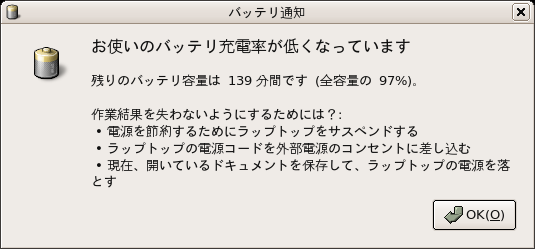
\includegraphics[width=0.8\hsize]{image200607/batterylo.png}

\subsubsection{$B%M%C%H%o!<%/$N@_Dj(B}

$BM-@~%M%C%H%o!<%/$O(B SKY2 $B$N%I%i%$%P$rMxMQ$7$^$9!#(B

$BL5@~%M%C%H%o!<%/$O!!(Bmadwifi $B$GBP1~$G$-$^$9!#(B
$B%$%s%9%H!<%kJ}K!$O2<5-$G$9!#(B

\begin{itemize}
  \item \texttt{sudo apt-get install madwifi-source madwifi-tools madwifi-doc}
  \item \texttt{sudo m-a prepare}
  \item \texttt{sudo m-a a-i madwifi}
  \item \texttt{sudo modprobe ath\_pci}
\end{itemize}

$BJ|$C$F$*$/$H(Bhotplug$B$K$h$j!"5/F0;~$K<+F0%m!<%I$5$l$FM-8z$K$J$j$^$9!#(B
\texttt{/etc/hotplug/blacklist.d/}$B$K%U%!%$%k$r:n@.$7!"2<5-$N$h$&$JFbMF$r(B
$BDI2C$7$F$*$/$H<jF0$G%m!<%I$7$J$$$HM-8z$K$J$i$J$$$h$&$K$G$-$^$9!#Ht9T5!$K(B
$B$N$k>l9g$J$I$N$?$a$K$OI,MW$+$b$7$l$^$;$s!#(B

\begin{commandline}
 ath_pci
\end{commandline}

$B0J2<!"%$%s%9%H!<%k;z$N%m%0$NNc$G$9!#(B

\begin{commandline}
 $ sudo apt-get install madwifi-source madwifi-tools madwifi-doc
 $ sudo m-a prepare
Getting source for kernel version: 2.6.17dancer
/lib/modules/2.6.17dancer/source $B$N%+!<%M%k%X%C%@$rMxMQ$G$-$^$9(B
symlink $B$r:n@.Cf(B...
apt-get install build-essential
$B%Q%C%1!<%8%j%9%H$rFI$_9~$s$G$$$^$9(B... $B40N;(B
$B0MB84X78%D%j!<$r:n@.$7$F$$$^$9(B... $B40N;(B
$B0J2<$N%Q%C%1!<%8$,?7$?$K%$%s%9%H!<%k$5$l$^$9(B:
  build-essential
$B%"%C%W%0%l!<%I(B: 0 $B8D!"?75,%$%s%9%H!<%k(B: 1 $B8D!":o=|(B: 0 $B8D!"J]N1(B: 94 $B8D!#(B
6916B $B$N%"!<%+%$%V$r<hF@$9$kI,MW$,$"$j$^$9!#(B
$BE83+8e$KDI2C$G(B 20.5kB $B$N%G%#%9%/MFNL$,>CHq$5$l$^$9!#(B
$B<hF@(B:1 http://ftp.jp.debian.org sid/main build-essential 11.2 [6916B]
6916B $B$r(B 0s $B$G<hF@$7$^$7$?(B (81.0kB/s)
$B%Q%C%1!<%8%U%#!<%k%I$rFI$_9~$s$G$$$^$9(B... $B40N;(B
$B%Q%C%1!<%8>uBV$rFI$_9~$s$G$$$^$9(B... $B40N;(B
$B%P%0%l%]!<%H$r<hF@$7$F$$$^$9(B... $B40N;(B
($B%G!<%?%Y!<%9$rFI$_9~$s$G$$$^$9(B ... $B8=:_(B 101852 $B8D$N%U%!%$%k$H%G%#%l%/%H%j$,%$%s%9%H!<%k$5$l$F$$$^$9!#(B)
(.../build-essential_11.2_i386.deb $B$+$i(B) build-essential $B$rE83+$7$F$$$^$9(B...
build-essential (11.2) $B$r@_Dj$7$F$$$^$9(B ...

$B40N;(B!
$ sudo m-a a-i madwifi
$B%Q%C%1!<%8%j%9%H$rFI$_9~$s$G$$$^$9(B... $B40N;(B
$B0MB84X78%D%j!<$r:n@.$7$F$$$^$9(B... $B40N;(B
madwifi-source $B$O$9$G$K:G?7%P!<%8%g%s$G$9!#(B
$B%"%C%W%0%l!<%I(B: 0 $B8D!"?75,%$%s%9%H!<%k(B: 0 $B8D!":o=|(B: 0 $B8D!"J]N1(B: 94 $B8D!#(B

1 $B%Q%C%1!<%8$K$D$$$F$N>pJs$r99?7$7$^$7$?(B
Extracting the package tarball, /usr/src/madwifi.tar.bz2, please wait...
\end{commandline}

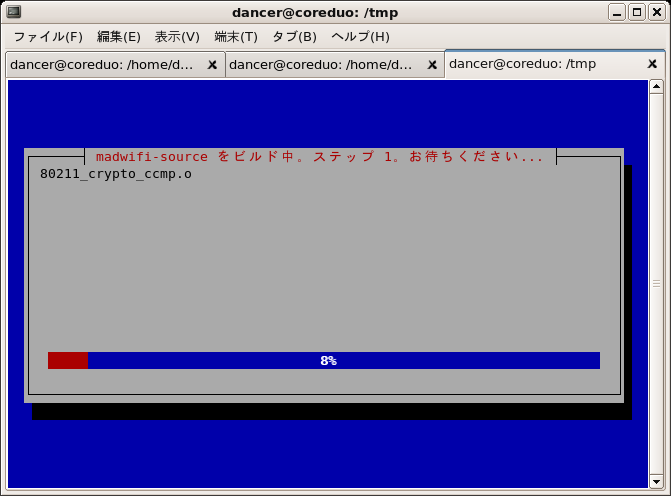
\includegraphics[width=0.8\hsize]{image200607/madwifi.png}

\begin{commandline}
/home/dancer/shared/git/madwifi-modules-2.6.17dancer_0.svnr1644.0.9.0-2+20060705_i386.deb $B$,40N;$7$^$7$?!#(B
$BL$A*Br%Q%C%1!<%8(B madwifi-modules-2.6.17dancer $B$rA*Br$7$F$$$^$9!#(B
($B%G!<%?%Y!<%9$rFI$_9~$s$G$$$^$9(B ... $B8=:_(B 101861 $B8D$N%U%!%$%k$H%G%#%l%/%H%j$,%$%s%9%H!<%k$5$l$F$$$^$9!#(B)
(.../madwifi-modules-2.6.17dancer_0.svnr1644.0.9.0-2+20060705_i386.deb $B$+$i(B) madwifi-modules-2.6.17dancer 
$B$rE83+$7$F$$$^$9(B...
madwifi-modules-2.6.17dancer (0.svnr1644.0.9.0-2+20060705) $B$r@_Dj$7$F$$$^$9(B ...

$ sudo modprobe ath_pci
$ lsmod | grep ath_pci
ath_pci                82212  0
ath_rate_sample        11776  1 ath_pci
wlan                  167132  4 wlan_scan_sta,ath_pci,ath_rate_sample
ath_hal               192208  3 ath_pci,ath_rate_sample
$ dmesg | tail -20
eth1: no IPv6 routers present
ath_hal: module license 'Proprietary' taints kernel.
ath_hal: 0.9.17.2 (AR5210, AR5211, AR5212, RF5111, RF5112, RF2413, RF5413)
wlan: 0.8.4.2 (svn r)
ath_rate_sample: 1.2 (svn r)
ath_pci: 0.9.4.5 (svn r)
Device `[PXS2]is not power manageable<6>ACPI: PCI Interrupt 0000:02:00.0[A] -> GSI 17 (level, low) -> IRQ 169
PCI: Setting latency timer of device 0000:02:00.0 to 64
wifi0: 11a rates: 6Mbps 9Mbps 12Mbps 18Mbps 24Mbps 36Mbps 48Mbps 54Mbps
wifi0: 11b rates: 1Mbps 2Mbps 5.5Mbps 11Mbps
wifi0: 11g rates: 1Mbps 2Mbps 5.5Mbps 11Mbps 6Mbps 9Mbps 12Mbps 18Mbps 24Mbps 36Mbps 48Mbps 54Mbps
wifi0: H/W encryption support: WEP AES AES_CCM TKIP
wifi0: mac 10.3 phy 6.1 radio 10.2
wifi0: Use hw queue 1 for WME_AC_BE traffic
wifi0: Use hw queue 0 for WME_AC_BK traffic
wifi0: Use hw queue 2 for WME_AC_VI traffic
wifi0: Use hw queue 3 for WME_AC_VO traffic
wifi0: Use hw queue 8 for CAB traffic
wifi0: Use hw queue 9 for beacons
wifi0: Atheros 5424: mem=0x90100000, irq=169

$ /sbin/ifconfig ath0
ath0      $B%j%s%/J}K!(B:$B%$!<%5!<%M%C%H(B  $B%O!<%I%&%'%"%"%I%l%9(B 00:16:CB:BA:76:E7 
          inet$B%"%I%l%9(B:192.168.22.42 $B%V%m!<%I%-%c%9%H(B:192.168.22.255 $B%^%9%/(B:255.255.255.0
          inet6$B%"%I%l%9(B: fe80::216:cbff:feba:76e7/64 $BHO0O(B:$B%j%s%/(B
          UP BROADCAST RUNNING MULTICAST  MTU:1500  Metric:1
          RX packets:1176 errors:0 dropped:0 overruns:0 frame:0
          TX packets:1607 errors:0 dropped:0 overruns:0 carrier:0
      $B>WFM(B(Collisions):0 TX$B%-%e!<D9(B:0 
          RX bytes:230678 (225.2 KiB)  TX bytes:1306390 (1.2 MiB)

\end{commandline}




\subsubsection{$B%j%b%3%s(B}

$B@V30@~$N%j%b%3%s$O;H$($k$h$&$G$9!#%+!<%M%kMQ$N%G%P%$%9%I%i%$%P$,B8:_$7$^(B
$B$9!#(B2.6.18$B0J9_$K$H$j$3$^$l$k$N$G$O$J$$$G$7$g$&$+!)(B
$B%f!<%66u4V$GMxMQ$G$-$k%I%i%$%P$O:n@.$7$F$*$-$^$7$?!#(B
\footnote{\url{http://www.netfort.gr.jp/~dancer/diary/daily/2006-Jul-12.html.ja}}

\subsubsection{iSight}

iSight $B$O(B linux-uvc$B%G%P%$%9$G$9!#(B
$B%U%!!<%`%&%'%"$N%m!<%I$,I,MW$G$9!#(B
$B<!$N<j=g$G%$%s%9%H!<%k$,$G$-$^$9!#(B

\begin{itemize}
 \item \texttt{apt-get install linux-uvc-tools linux-uvc-source}
 \item \texttt{module-assistant auto-install linux-uvc}
\end{itemize}

$B%"%W%j%1!<%7%g%s$O(Bekiga$B$J$I$rMxMQ$7$^$7$g$&!#(B
v4l2$B%G%P%$%9$J$N$G!"(Bv4l2$BBP1~$N%=%U%H%&%'%"$,I,MW$G$9!#(B

\begin{itemize}
 \item \texttt{apt-get install ekiga libpt-plugins-v4l2}
\end{itemize}

$B<B:]$K%m!<%I$9$k$K$O!"(BMac OS X$B$N%G%P%$%9%I%i%$%P$KF~$C$F$$$k%U%!!<%`%&%'(B
$B%"$r%m!<%I$7$F$+$i%b%8%e!<%k$r%m!<%I$7$^$9!#%I%i%$%P$N$"$k>l=j$N%G%#%l%/(B
$B%H%j3,AX$,?<$$$N$GCm0U!#(B

\begin{itemize}
 \item \texttt{sudo mount /dev/sda2 /mnt/macosx}
 \item \texttt{sudo macbook-isight-firmware-loader \\
       /mnt/mac/System/Library/Extensions/IOUSBFamily.kext/Contents/PlugIns($B<!$N9T$KB3$/(B)\\/AppleUSBVideoSupport.kext/Contents/MacOS/AppleUSBVideoSupport}
 \item \texttt{modprobe uvcvideo}
\end{itemize}


\subsubsection{$BL$3NG'$N%G%P%$%9!"<jK!(B}

Debian$B$r<+F05/F0$5$;$kJ}K!$,$o$+$j$^$;$s!"(BrEFIt$B$O%G%U%)%k%H$G$O!"(BMacOSX
$B$b$7$/$O(BeLILO$B$r5/F0$7$h$&$H$7$F$7$^$$$^$9!#(BeLILO$B$r5/F0$9$k$H5/F0$G$-$J$$!#(B
$BM%@hEY$NJQ99$O$I$&$d$C$?$i$h$$$N$+!"$H$$$&$N$,$$$^$$$AITL@$G$9!#(B

$B%5%9%Z%s%I$NJ}K!!#(B

$B%9%j!<%W$NJ}K!!#(B

CD-R$B$NF0:n$O$^$@3NG'$7$F$$$^$;$s!#(BPATA$B%Q%C%A$,I,MW$H$$$&1=$G$9!#(B

\begin{commandline}
 
 # cdrecord -scanbus
 scsibus0:
        0,0,0     0) *
        0,1,0     1) 'ATA     ' 'ST98823AS       ' '7.01' Disk
        0,2,0     2) *
        0,3,0     3) *
        0,4,0     4) *
        0,5,0     5) *
        0,6,0     6) *
        0,7,0     7) *
\end{commandline}

$B%P%C%/%i%$%H$N@)8f$,$G$-$k%I%i%$%P$O:n@.$5$l$F$$$k$N$G!"(B2.6.18$B$+(B19$B$/$i$$(B
$B$K$OF~$k$N$G$O$J$$$G$7$g$&$+!#(B

bluetooth$B$K$D$$$F$OL$D4::!#(B

\subsection{$BH/I=MzNr(B}

$BK\;qNA$O2<5-$N>l=j$G$NH/I=;qNA$H$7$F:n@.$5$l$?$b$N$G$9!#(B
$BFbMF$K$D$$$F$O?o;~99?7$7$J$,$i!"$$$/$D$+$N>l=j$GH/I=$7$F$$$^$9!#(B

\begin{itemize}
 \item 2006$BG/(B7$B7n(B2$BF|(B $B=)MU86!"(BCodeFestAkihabara  2006:$B!!:G=*Js9p(B
 \item 2006$BG/(B7$B7n(B6$BF|(B $B7CHf<w!"(BSGI$B%[!<%k!"%+!<%M%kFI=q2q(B: mixi.jp $B$NOC$NA0:B(B
 \item 2006$BG/(B7$B7n(B15$BF|(B $BKL3$F;!"(BOSC-Do 2006: $B!V(BDebian$BJY6/2q!W$N%;%C%7%g%s(B
 \item 2006$BG/(B7$B7n(B29$BF|(B $BF|!9C+!"(BTLUG: $B!V(BMacBook$B$K(BMac OS X$B$H(BDebian$B$r(B
       dual-boot$B$G%$%s%9%H!<%k!W(B
\end{itemize}

\subsection{$B;29MJ88%(B}

$B%U%!!<%`%&%'%"$N(B bootcamp$B!!$^$o$j$N3+H/$N1F6A$G!"$[$H$s$I$N(Bweb$B>e$N<j=g$r(B
$B=q$$$F$"$kJ88%$O8=:_$N;~E@$G<j=g$,8E$/$J$C$F$$$k$N$G!";29M$K$J$i$J$$>l9g(B
$B$,B?$$$G$9$,!":#8e99?7$5$l$k$+$b$7$l$^$;$s!#(B

\begin{itemize}
 \item MacBook Developer Note: MacBook$B$NO@M}9=@.?^!"%O!<%I%&%'%"$N354Q$,2r@b$5$l$F$$$^$9!#!!(B
       \url{http://developer.apple.com/documentation/HardwareDrivers/Conceptual/MacBook_0605/index.html}
 \item $B@V30@~%j%b!<%H%3%s%H%m!<%kMQ!"(BIR Receiver$B!!%Q%C%A(B
       \url{http://sourceforge.net/mailarchive/message.php?msg_id=16309282}
       \url{http://www.madingley.org/macmini/kernel/ir.patch}
 \item $B@V30@~%j%b!<%H%3%s%H%m!<%k$G(BXPDF$B%W%l%<%s%F!<%7%g%s$9$k%Q%C%A!#(B
       \url{http://www.netfort.gr.jp/~dancer/diary/daily/2006-Jul-12.html.ja#2006-Jul-12-00:00:06}
 \item MacBook $B$N;EMM!'!!4JC1$K35MW$@$1$,@bL@$5$l$F$$$^$9!#(B
       \url{http://support.apple.com/specs/macbook/macbook.html}
 \item iSight (IEEE1394 $B30It%G%P%$%9(B)$B$N%W%m%0%i%_%s%0%,%$%I!!(B
       \url{http://developer.apple.com/documentation/Hardware/Conceptual/iSightProgGuide/
iSightProgGuide.pdf}
 \item bluetooth $B$N%I%-%e%a%s%H!'!!(B\url{http://developer.apple.com/documentation/HardwareDrivers/Conceptual/HWTech_Bluetooth/index.html#//apple_ref/doc/uid/TP40003032}
 \item mactel linux$B$N%Z!<%8!!(B\url{http://mactel-linux.org/}$B!"(B
       $B$3$3$+$i$?$I$l$k%a!<%j%s%0%j%9%H$GM-MQ$J>pJs$,8r49$5$l$F$$$^$9!#(B
 \item rEFIt$B$N%Z!<%8!!(B\url{http://refit.sourceforge.net/}
 \item \url{http://sharealike.org/index.php?m=200605}
 \item $B%P%C%/%i%$%H@)8f(B
       \url{http://modular.math.washington.edu/macbook/backlight/}
 \item Ubuntu$B$N%$%s%9%H!<%k$K$D$$$F$N$^$H$a%Z!<%8(B
       \url{http://desrt.mcmaster.ca/macbook.xhtml}
 \item Gentoo $B$N>pJs%Z!<%8!!(B
       \url{http://gentoo-wiki.com/HARDWARE_Apple_MacBook}
 \item MadWifi Wiki
       \url{http://madwifi.org/wiki/UserDocs/Distro/Debian/MadWifing}
 \item Macbook Pro build-in iSight
       \url{http://blogs.gnome.org/view/rbultje/2006/07/08/0}
 \item linux usb video class, linux-uvc
       \url{http://linux-uvc.berlios.de}
 \item Debian wiki MacBook \url{http://wiki.debian.org/MacBook}
\end{itemize}

\dancersection{$B<!2s(B}{}

$BL$Dj$G$9!#(B
$BFbMF$OK\F|7hDjM=Dj$G$9!#(B

$B;22C<TJg=8$O$^$?8eDx!#(B

\newpage

\vspace*{15cm}
\hrule
\vspace{2mm}

\includegraphics[width=2cm]{image200502/openlogo-nd.eps}
\noindent \Large \bf Debian $BJY6/2q;qNA(B\\ \\
\noindent \normalfont 2006$BG/(B7$B7n(B15$BF|(B \hspace{5mm}  $B=iHGBh(B1$B:~H/9T(B\\
\noindent \normalfont $BEl5~%(%j%"(B Debian $BJY6/2q(B $B!JJT=8!&0u:~!&H/9T!K(B\\
\hrule

\end{document}
